%package list
\documentclass{article}
\usepackage[top=3cm, bottom=3cm, outer=3cm, inner=3cm]{geometry}
\usepackage{multicol}
\usepackage{graphicx}
\usepackage{url}
%\usepackage{cite}
\usepackage{hyperref}
\usepackage{array}
%\usepackage{multicol}
\newcolumntype{x}[1]{>{\centering\arraybackslash\hspace{0pt}}p{#1}}
\usepackage{natbib}
\usepackage{pdfpages}
\usepackage{multirow}
\usepackage[utf8]{inputenc}
\usepackage[normalem]{ulem}
\useunder{\uline}{\ul}{}
\usepackage{svg}
\usepackage{xcolor}
\usepackage{listings}
\lstdefinestyle{ascii-tree}{
    literate={├}{|}1 {─}{--}1 {└}{+}1 
  }
\lstset{basicstyle=\ttfamily,
  showstringspaces=false,
  commentstyle=\color{red},
  keywordstyle=\color{blue}
}
%\usepackage{booktabs}
\usepackage{caption}
\usepackage{subcaption}
\usepackage{float}
\usepackage{array}

\newcolumntype{M}[1]{>{\centering\arraybackslash}m{#1}}
\newcolumntype{N}{@{}m{0pt}@{}}


%%%%%%%%%%%%%%%%%%%%%%%%%%%%%%%%%%%%%%%%%%%%%%%%%%%%%%%%%%%%%%%%%%%%%%%%%%%%
%CREACIÓN DE VARIABLE
\newcommand{\itemEmail}{jcondoripin@unsa.edu.pe}
\newcommand{\itemStudent}{Juan José Condori Pinto}
\newcommand{\itemCourse}{Programación Web 2}
\newcommand{\itemCourseCode}{1702122}
\newcommand{\itemSemester}{III}
\newcommand{\itemUniversity}{Universidad Nacional de San Agustín de Arequipa}
\newcommand{\itemFaculty}{Facultad de Ingeniería de Producción y Servicios}
\newcommand{\itemDepartment}{Departamento Académico de Ingeniería de Sistemas e Informática}
\newcommand{\itemSchool}{Escuela Profesional de Ingeniería de Sistemas}


%AQUIIII: CAMBIA LA INFO DEL LAB
\newcommand{\itemAcademic}{2023 - A}
\newcommand{\itemInput}{26 Junio 2023}
\newcommand{\itemOutput}{03 Julio 2023}
\newcommand{\itemPracticeNumber}{08}
\newcommand{\itemTheme}{Django Rest Framework}
%%%%%%%%%%%%%%%%%%%%%%%%%%%%%%%%%%%%%%%%%%%%%%%%%%%%%%%%%%%%%%%%%%%%%%%%%%%%


%PARA EL PIE DE PÁGINA
\usepackage{fancyhdr}
\pagestyle{fancy}
\fancyhf{}
\setlength{\headheight}{30pt}
\renewcommand{\headrulewidth}{1pt}
\renewcommand{\footrulewidth}{1pt}
\fancyhead[L]{\raisebox{-0.2\height}{\includegraphics[width=3cm]{img/logo_episunsa.png}}}
\fancyhead[C]{\fontsize{7}{7}\selectfont	\itemUniversity \\ \itemFaculty \\ \itemDepartment \\ \itemSchool \\ \textbf{\itemCourse}}
\fancyhead[R]{\raisebox{-0.2\height}{\includegraphics[width=1.2cm]{img/logo_abet}}}
\fancyfoot[L]{Estudiante Juan José Condori Pinto}
\fancyfoot[C]{\itemCourse}
\fancyfoot[R]{Página \thepage}

% para el codigo fuente
\usepackage{listings}
\usepackage{color, colortbl}
\definecolor{dkgreen}{rgb}{0,0.6,0}
\definecolor{gray}{rgb}{0.5,0.5,0.5}
\definecolor{mauve}{rgb}{0.58,0,0.82}
\definecolor{codebackground}{rgb}{0.95, 0.95, 0.92}
\definecolor{tablebackground}{rgb}{0.8, 0, 0}

\lstset{frame=tb,
	language=bash,
	aboveskip=3mm,
	belowskip=3mm,
	showstringspaces=false,
	columns=flexible,
	basicstyle={\small\ttfamily},
	numbers=none,
	numberstyle=\tiny\color{gray},
	keywordstyle=\color{blue},
	commentstyle=\color{dkgreen},
	stringstyle=\color{mauve},
	breaklines=true,
	breakatwhitespace=true,
	tabsize=3,
	backgroundcolor= \color{codebackground},
}


\begin{document}
        %CARÁTULA
        \vspace*{10px}
    	
        \begin{center}	
            \fontsize{17}{17} \textbf{ Informe de Laboratorio \itemPracticeNumber}
        \end{center}
        \centerline{\textbf{\Large Tema: \itemTheme}}
        %\vspace*{0.5cm}	
    
        \begin{flushright}
    	\begin{tabular}{|M{2.5cm}|N|}
    		\hline 
    		\rowcolor{tablebackground}
    		\color{white} \textbf{Nota} \\
    		\hline 
    			\\[30pt]
    		\hline 			
    	\end{tabular}
        \end{flushright}	

	\begin{table}[H]
		\begin{tabular}{|x{4.7cm}|x{4.8cm}|x{4.8cm}|}
			\hline 
			\rowcolor{tablebackground}
			\color{white} \textbf{Estudiante} & \color{white}\textbf{Escuela}  & \color{white}\textbf{Asignatura}   \\
			\hline 
			{\itemStudent \par \itemEmail} & \itemSchool & {\itemCourse \par Semestre: \itemSemester \par Código: \itemCourseCode}     \\
			\hline 			
		\end{tabular}
	\end{table}		
	
	\begin{table}[H]
		\begin{tabular}{|x{4.7cm}|x{4.8cm}|x{4.8cm}|}
			\hline 
			\rowcolor{tablebackground}
			\color{white}\textbf{Laboratorio} & \color{white}\textbf{Tema}  & \color{white}\textbf{Duración}   \\
			\hline 
			\itemPracticeNumber & \itemTheme & 04 horas   \\
			\hline 
		\end{tabular}
	\end{table}
	
	\begin{table}[H]
		\begin{tabular}{|x{4.7cm}|x{4.8cm}|x{4.8cm}|}
			\hline 
			\rowcolor{tablebackground}
			\color{white}\textbf{Semestre académico} & \color{white}\textbf{Fecha de inicio}  & \color{white}\textbf{Fecha de entrega}   \\
			\hline 
			\itemAcademic & \itemInput &  \itemOutput  \\
			\hline 
		\end{tabular}
	\end{table}

\section{Tarea}
        \begin{itemize}
            \item En sus grupos de trabajo correspondientes. Elabore un servicio web que tenga un CRUD con el uso de este framework.
            \item Create - POS        
            \item Read - GET
            \item Update - PUT
            \item Delete - DELETE
        \end{itemize}

    La aplicacion y servicio creado para este laboratorio se estará basando en el manejo de una tabla 'Employees', siendo un CRUD basico con interfaz de api y frontend desarrollado en Angular
        
    \subsection{Commits}
        \begin{figure}
            \centering
            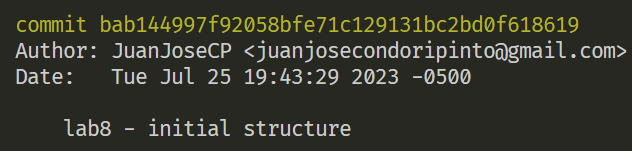
\includegraphics{img/commit0.png}
            \caption{Commit para definicion de estructura inicial del proyecto de backend}
            \label{fig:enter-label}
        \end{figure}
        \begin{figure}
            \centering
            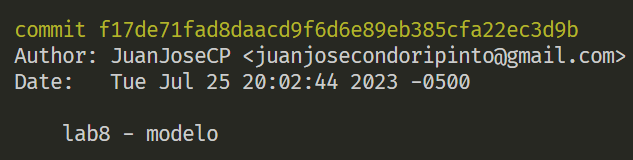
\includegraphics{img/commit1.png}
            \caption{Commit para definicion de modelo Employee}
            \label{fig:enter-label}
        \end{figure}
        \begin{figure}
            \centering
            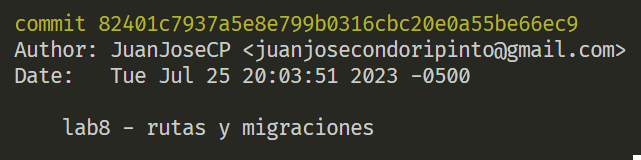
\includegraphics{img/commit2.png}
            \caption{Commit para definicion de rutas y migraciones}
            \label{fig:enter-label}
        \end{figure}
        \begin{figure}
            \centering
            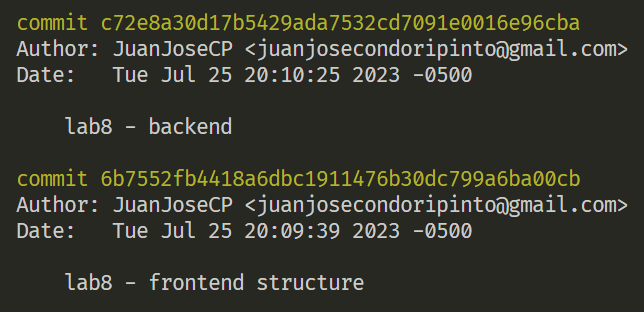
\includegraphics{img/commit3.png}
            \caption{Commit para separacion de front y backend}
            \label{fig:enter-label}
        \end{figure}
        \begin{figure}
            \centering
            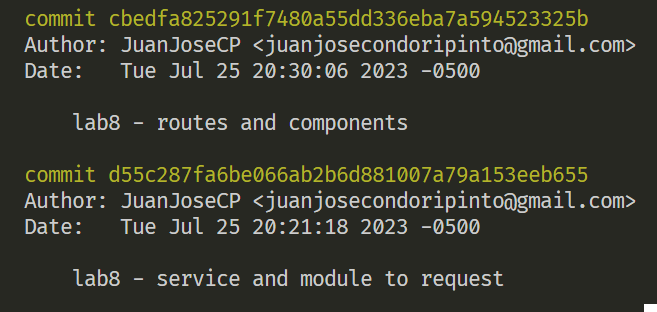
\includegraphics{img/commit4.png}
            \caption{Commit para creacion de rutas en Angular, componentes y servicios para peticiones Http}
            \label{fig:enter-label}
        \end{figure}
        \begin{figure}
            \centering
            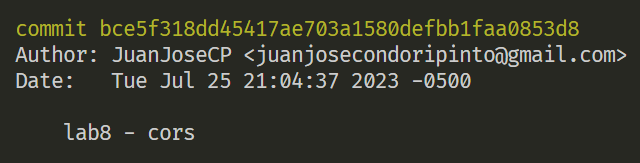
\includegraphics{img/commit5.png}
            \caption{Commit para implementacion de middleware cors en django (comunicacion con frontend)}
            \label{fig:enter-label}
        \end{figure}
        \begin{figure}
            \centering
            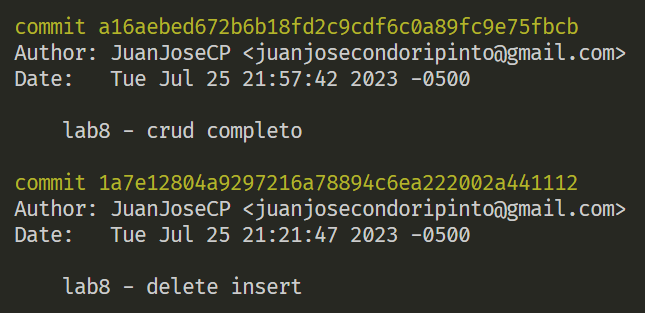
\includegraphics{img/commit6.png}
            \caption{Commit para metodos crud en frontend}
            \label{fig:enter-label}
        \end{figure}
    \newpage
        
    \subsection{Estructura y codigo}
        \begin{figure}[ht]
            \centering
            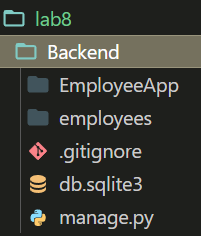
\includegraphics{img/img0.png}
            \caption{Estructura de backend}
            \label{fig:enter-label}
        \end{figure}
        \textbf{Aqui podemos ver la estructura del proyecto EmployeeApp en django, las apis estaran desarrolladas con rest\_framework}
        
        \begin{figure}[ht]
            \centering
            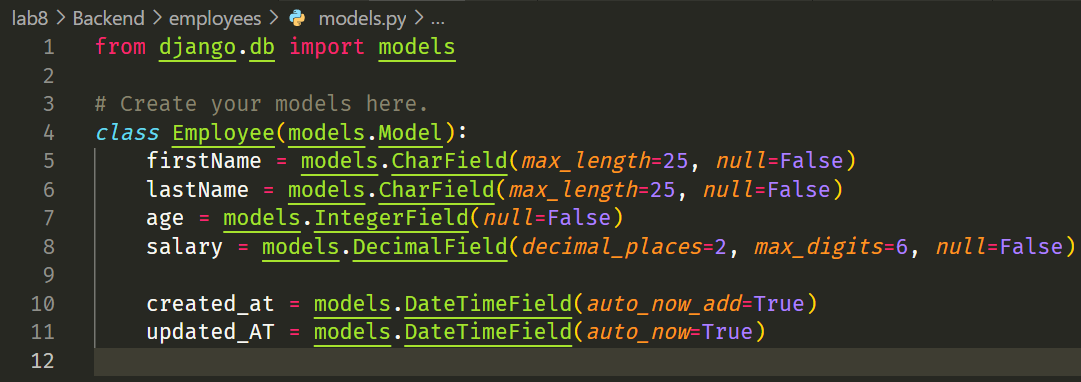
\includegraphics[scale=0.5]{img/img1.png}
            \caption{Modelo employee}
            \label{fig:enter-label}
        \end{figure}
        \textbf{Como podemos ver, el modelo de empleado posee algunos campos basicos para su manejo, tales como nombres, apellidos, edad y salario, ademas de las fechas de actualizacion}

        
        \begin{figure}[ht]
            \centering
            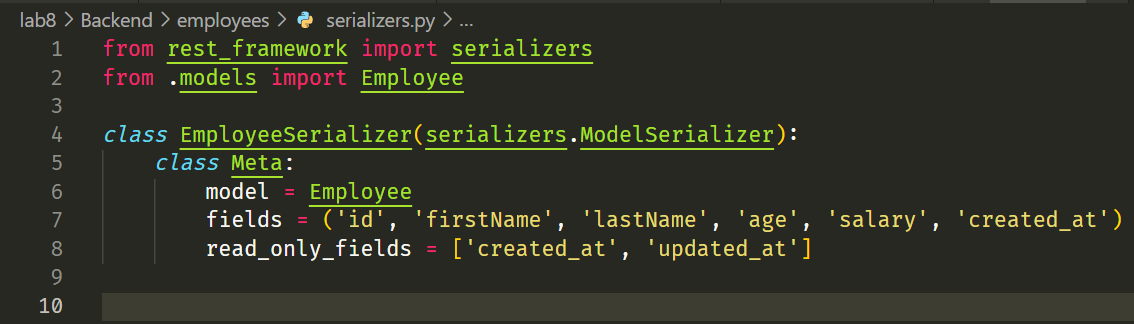
\includegraphics[scale=0.5]{img/img2.png}
            \caption{Employee serializer}
            \label{fig:enter-label}
        \end{figure}
        \textbf{Esta clase permite serializar el modelo de empleado para que sus datos puedan ser leidos por el navegador y enviados como respuesta}
        \newpage
        
        \begin{figure}[ht]
            \centering
            
\includegraphics{img/img3.png}
            \caption{ViewSet para api}
            \label{fig:enter-label}
        \end{figure}
        \textbf{El ViewSet es una vista heredada de rest framework que permite la creacion interfaces para las apis, en este caso, el modelo a serializar sera el de Employee y trabajara sobre todos sus registros}

        
        \begin{figure}[ht]
            \centering
            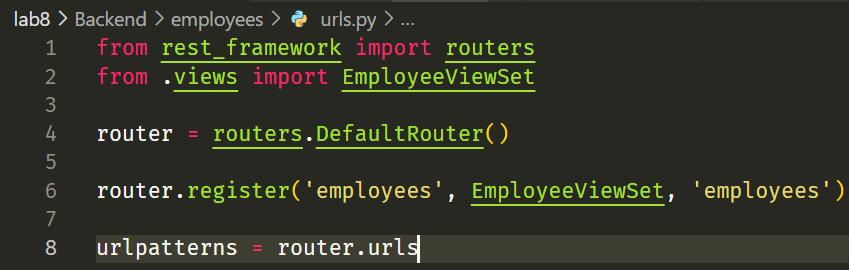
\includegraphics[scale=0.7]{img/img4.png}
            \caption{Urls app}
            \label{fig:enter-label}
        \end{figure}
        \textbf{Con routers podemos registrar las vistas de api que tenemos disponibles, en este caso, la de empleados, esto permitira la creacion de una interfaz para el manejo de la api}
        \newpage
        
        \begin{figure}[ht]
            \centering
            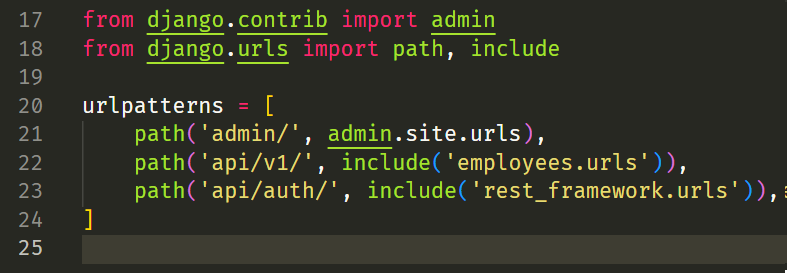
\includegraphics[scale=0.5]{img/img5.png}
            \caption{Registro de urls de apis en proyecto}
            \label{fig:enter-label}
        \end{figure}

        \begin{figure}[ht]
            \centering
            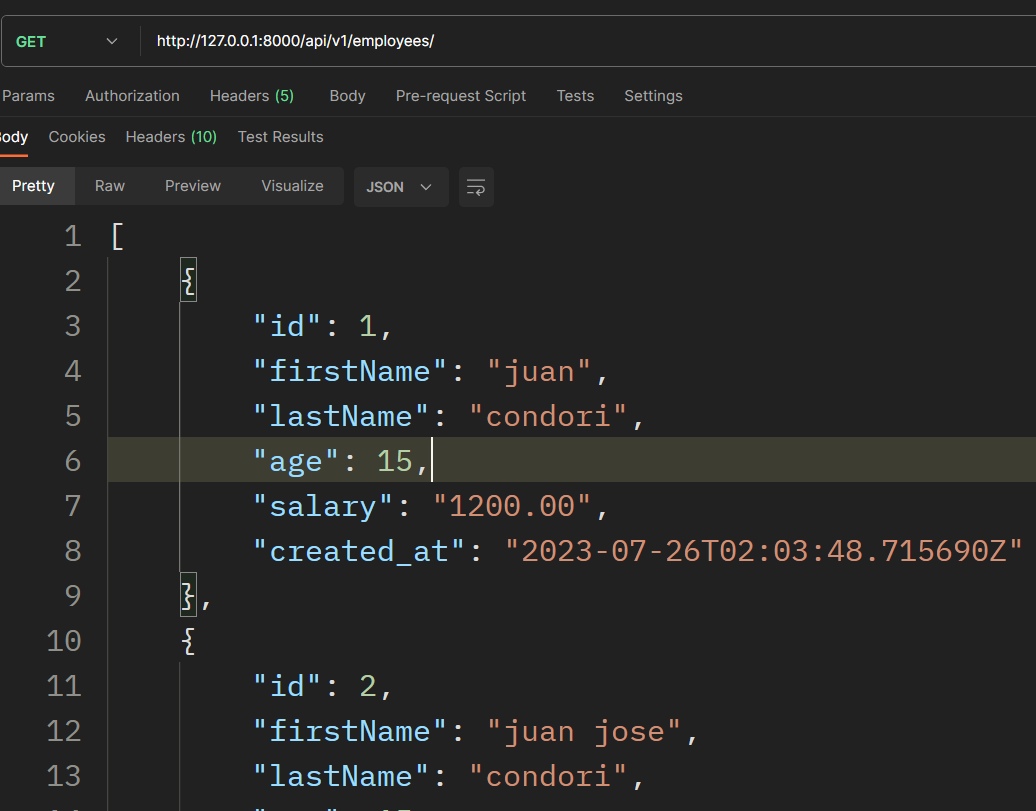
\includegraphics[scale=0.5]{img/img6.png}
            \caption{Prueba de api en Postman}
            \label{fig:enter-label}
        \end{figure}
        \textbf{Una forma de comprobar el funcionamiento de las apis es a traves de Postman, donde podemos hacer todo tipo de peticiones, en este caso, se inserto con anterioridad algunos registros de empleados}
        
        \begin{figure}[ht]
            \centering
            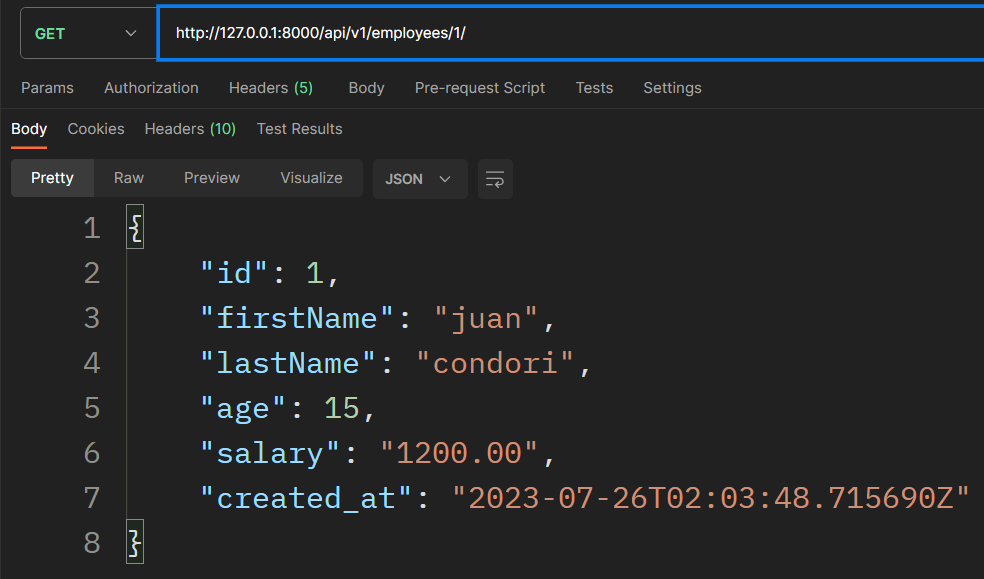
\includegraphics[scale=0.5]{img/img7.png}
            \caption{Prueba de api GET con parametro en Postman}
            \label{fig:enter-label}
        \end{figure}
    \newpage

    \subsection{Front end}
        \begin{figure}[ht]
            \centering
            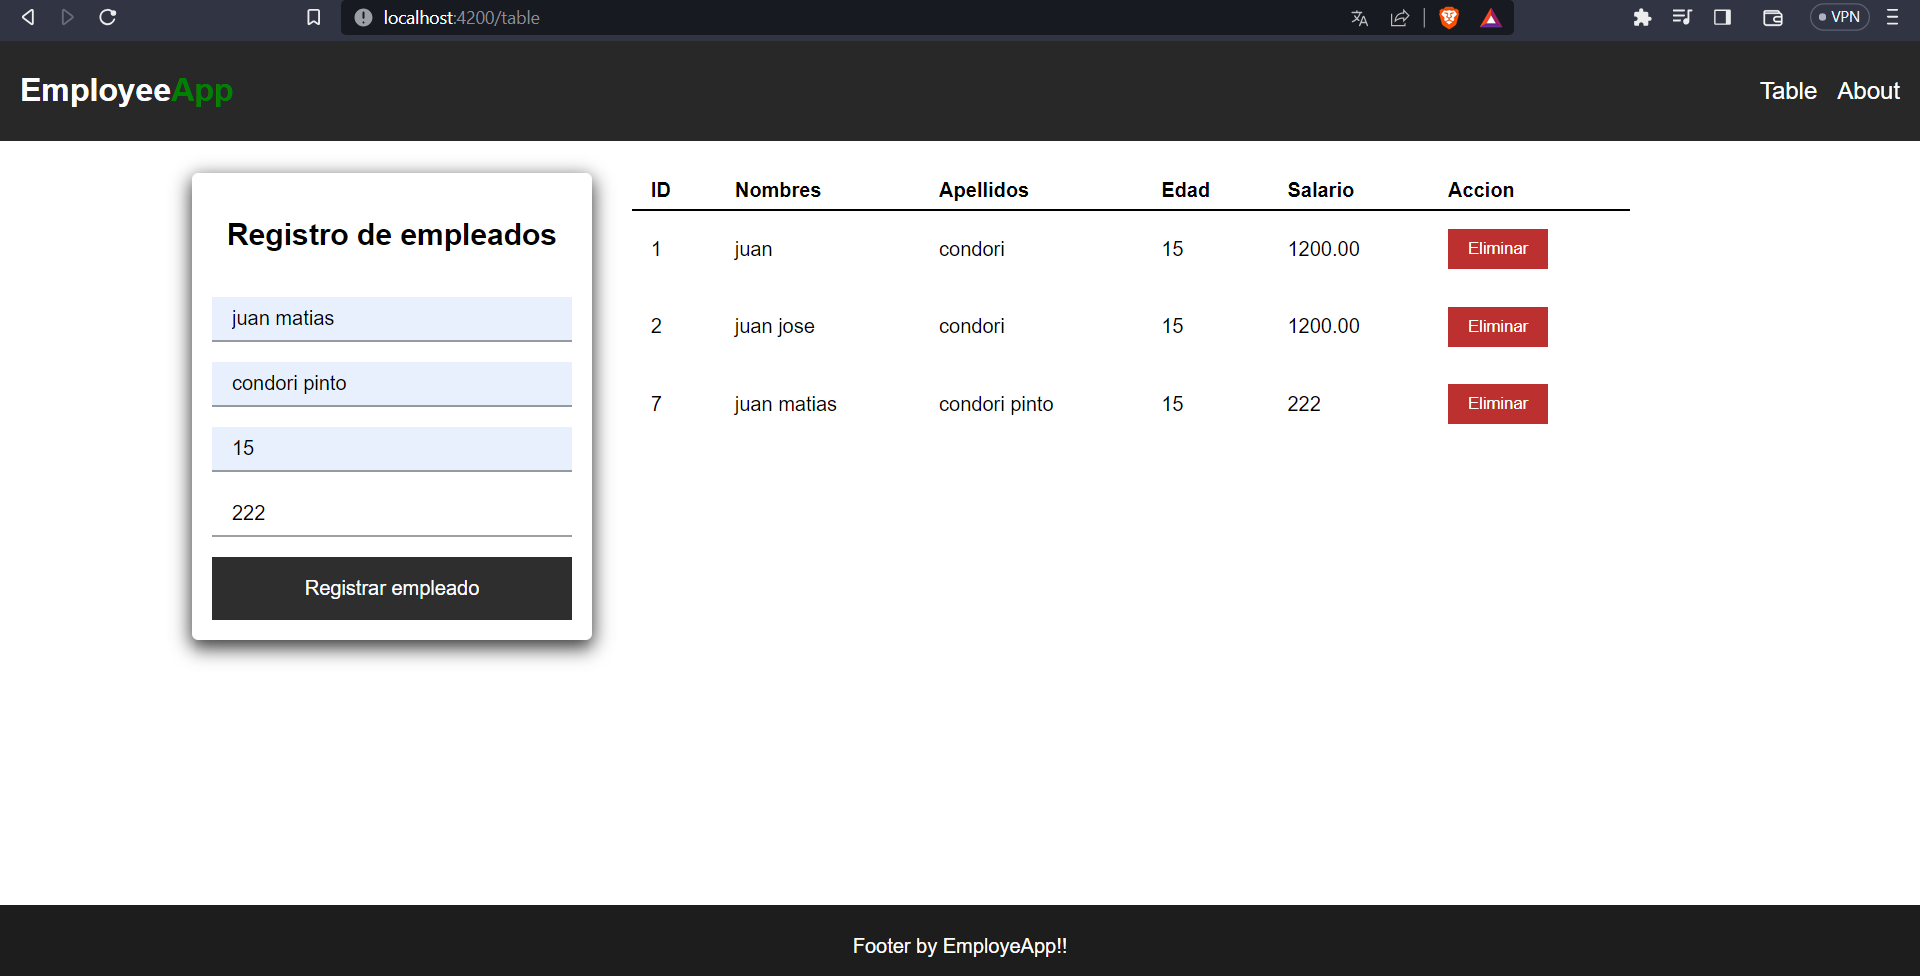
\includegraphics[scale=0.3]{img/img8.png}
            \caption{Front end index}
            \label{fig:enter-label}
        \end{figure}
        \textbf{En Angular, se desarrollo una interfaz para el consumo de la api creada con anterioridad, como podemos observar, esta es la vista general de la tabla Employees, de momento son 3 registros y podemos ir insertando algunos mas}
        \newpage
        
        \begin{figure}[ht]
            \centering
            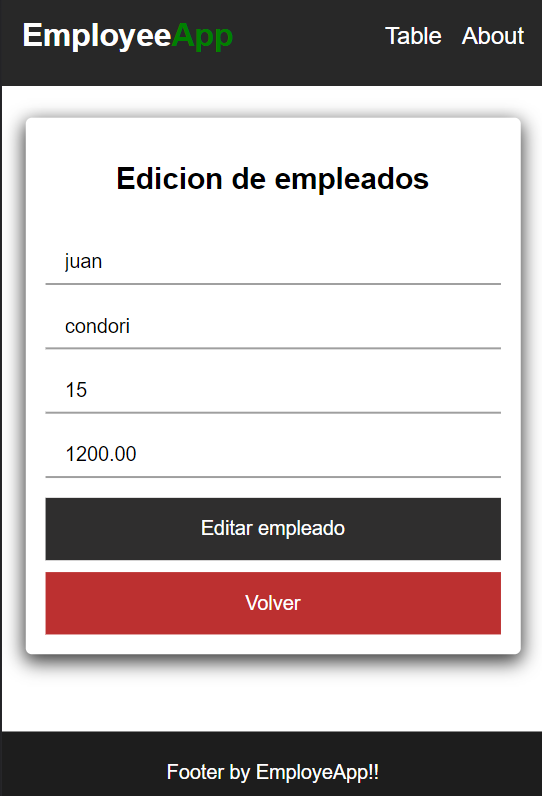
\includegraphics[scale=0.4]{img/img9.png}
            \caption{Edicion sobre tabla de Employees}
            \label{fig:enter-label}
        \end{figure}
        \textbf{Al dar click en cualquier fila de la tabla esta nos redireccionara a la vista de edicion del empleado seleccionado}
        
        \begin{figure}[ht]
            \centering
            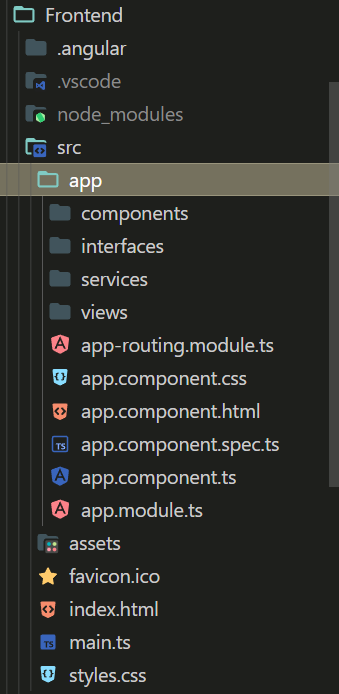
\includegraphics[scale=0.5]{img/img10.png}
            \caption{Estructura de proyecto frontend}
            \label{fig:enter-label}
        \end{figure}
        \textbf{Al dar click en cualquier fila de la tabla esta nos redireccionara a la vista de edicion del empleado seleccionado}

    \newpage
    \subsection{Comunicacion con backend}
            \begin{lstlisting}[caption=Servicio EmployeeService]
            import { Injectable } from '@angular/core';
            import { Employee } from '../interfaces/Employee';
            
            import { Observable } from 'rxjs';
            import { HttpClient } from '@angular/common/http';
            
            @Injectable({
              providedIn: 'root'
            })
            export class EmployeeServiceService {
            
              private urlApi = 'http://127.0.0.1:8000/api/v1/';
              public employees !: Employee[]
            
              constructor(private httpClient : HttpClient) {
                console.log('Using the data Employee service');
              }
            
              index() : Observable<Employee[]> {
                return this.httpClient.get<Employee[]>(`${this.urlApi}employees/`)
              }
            
              create(data : Employee) : Observable<any> {
                return this.httpClient.post(`${this.urlApi}employees/`, data)
              }
            
              show(id : number) : Observable<Employee>{
                return this.httpClient.get<Employee>(`${this.urlApi}employees/${id}/`)
              }
            
              update(id: number, employee: Employee) : Observable<any> {
                return this.httpClient.put(`${this.urlApi}employees/${id}/`, employee)
              }
            
              delete(id: number) : Observable<any> {
                return this.httpClient.delete(`${this.urlApi}employees/${id}/`)
              }
            
            }
            \end{lstlisting}
        \textbf{La libreria HttpClient de angular permite la comunicacion con el backend, como podemos observar se esta haciendo uso de los 4 metodos basicos para el CRUD, se emplean los observables para ejecutar dichos metodos cuando sea necesario dentro de una de las vistas implementadas}
    
\section{\textcolor{red}{Rubricas}}
        \subsection{\textcolor{red}{Rubrica para entregable Informe}}
            \begin{table}[ht]
                \centering
                \caption{Rúbrica para tipo de informe}
                \begin{tabular}{
                        |p{2.5cm}
                        |p{6cm}
                        |p{2cm}
                        |p{2cm} |}
                    \hline
                        \multicolumn{2}{|c|}{\textbf{Informe}} & \centerline{\textbf{Cumple}} & \centerline{\textbf{No cumple}} \\
                    \hline
                        \textbf{\textcolor{red}{Latex}} & \textcolor{blue}{El informe esta en formato PDF desde Latex, con un formato limpio (buena presentación) y facil de leer.} & \centerline{20} & \centerline{0} \\
                    \hline
                        \textbf{MarkDown} & El informe esta en formato PDF desde MarkDown README.md, con un formato limpio (buena presentacion) y facil de leer. & \centerline{17} & \centerline{0}\\
                    \hline
                        \textbf{MS Word} & El informe esta en formato PDF desde plantilla MS Word, con un formato limpio (buena presentacion) y facil de leer. & \centerline{15} & \centerline{0}\\
                    \hline
                        \textbf{Observaciones} & Por cada observacion se le descontara puntos. & \centerline{-} & \centerline{-}\\
                    \hline
                    \end{tabular}
                \label{tab:tab1}
            \end{table}
        \newpage
        \subsection{\textcolor{red}{Rubrica para el contenido del Informe y demostracion}}
            \begin{itemize}
                \item El alumno debera marcar o dejar en blanco en las celdas de la columna Checklist, deacuerdo a si cumplio o no con el ́ıtem correspondiente.
                \item Si un alumno supera la fecha de entrega, su calificacion siempre sera sobre la nota mınima aprobada, siempre y cuando cumpla con todos lo items.
                \item El alumno debe autocalificarse en la columna Estudiante de acuerdo a la tabla de calificacion de niveles de desempeño:
            \end{itemize}
            \begin{table}[ht]
                \centering
                \caption{Niveles de desempeño}
                \begin{tabular}{
                        >{\centering\arraybackslash}m{1.2cm}
                        >{\centering\arraybackslash}m{3cm}
                        >{\centering\arraybackslash}m{3cm}
                        >{\centering\arraybackslash}m{3cm}
                        >{\centering\arraybackslash}m{3cm}}
                    \hline
                    \multicolumn{5}{c}{Nivel} \\
                    \hline
                    \textbf{Puntos} & Insatisfactorio 25\% & En Proceso 50\% & Satisfactorio 75\% & Sobresaliente 100\% \\
                    \textbf{2.0} & 0.5 & 1.0 & 1.5 & 2.0 \\
                    \textbf{4.0} & 1.0 & 2.0 & 3.0 & 4.0 \\
                    \hline
                \end{tabular}
                \label{tab:tab2}
            \end{table}
            \begin{table}[]
                \centering
                \caption{Rubrica para contenido del Informe y demostracion}
                \begin{tabular}{
                    |m{2.5cm}
                    |m{7cm}
                    |>{\centering\arraybackslash}m{1cm}
                    |>{\centering\arraybackslash}m{1.2cm}
                    |>{\centering\arraybackslash}m{1.5cm}
                    |>{\centering\arraybackslash}m{1.2cm}|}
                    
                    \hline
                    \multicolumn{2}{|c|}{Contenido y demostracion} & Puntos & Checklist & Estudiante & Profesor \\
                    \hline
                    \textbf{1. GitHub} & Hay enlace URL activo del directorio para el laboratorio hacia su repositorio GitHub con codigo fuente terminado y facil de revisar. & 2 & X & 2 &   \\
                    \hline
                    \textbf{2. Commits} & Hay capturas de pantalla de los commits mas importantes con sus explicaciones detalladas. (El profesor puede preguntar para refrendar calificacion). & 4 & X & 3 &   \\
                    \hline
                    \textbf{3. Código fuente} & Hay porciones de codigo fuente importantes con numeracion y explicaciones detalladas de sus funciones. & 2 & X & 1 &   \\
                    \hline
                    \textbf{4. Ejecucion} & Se incluyen ejecuciones/pruebas del codigo fuente explicadas gradualmente. & 2 & X & 2 &   \\
                    \hline
                    \textbf{5. Pregunta} & Se responde con completitud a la pregunta formulada en la tarea. (El profesor puede preguntar para refrendar calificacion). & 2 & X & 2 &   \\
                    \hline
                    \textbf{6. Fechas} & Las fechas de modificacion del codigo fuente estan dentro de los plazos de fecha de entrega establecidos. & 2 & X & 2 &   \\
                    \hline
                    \textbf{7. Ortografia} & El documento no muestra errores ortograficos. & 2 & X & 2 &   \\
                    \hline
                    \textbf{8. Madurez} & El Informe muestra de manera general una evolucion de la madurez del codigo fuente, explicaciones puntuales pero precisas y un acabado impecable. (El profesor puede preguntar para refrendar calificacion). & 4 & X & 4 &   \\
                    \hline
                    \multicolumn{2}{|c|}{Total} & 20 &  & 18 & \\
                    \hline
                \end{tabular}
                \label{tab:tab3}
            \end{table}
\end{document}  